\chapter{関連研究}\label{ch:rel_res}

偽情報および偽情報の自動検出(真偽分類)は,対象にスパム\cite{shen2017discovering}や風評\cite{7023340},そして虚偽広告\cite{Huang:2017:DFO:3041021.3054233}を含めると新しいトピックではない.
\cref{ch:introduction}の通り,本研究はこれまでの研究\cite{Born2017-11-02,Shu:2017:FND:3137597.3137600,Ruchansky:2017:CHD:3132847.3132877,Wang:2018:EEA:3219819.3219903}に倣い,人を混乱させ惑わすために意図的・意識的に作られたウソ、虚偽の情報を偽情報と定義する.
なお、関連する単語として誤情報(誤報、misinformation)もあるが、これは勘違いや誤解により拡散された間違った情報を指すものとして区別されている\cite{Born2017-11-02,gov2024}。

本章では、偽情報の自動検出を行う研究で事実確認を行うファクトチェックの補助と情報生成技術の発展、偽情報の自動検出を通して既存研究が抱える問題点を指摘する。


\section{ファクトチェックの補助}
ファクトチェックを補助することが目的である研究は数多く,実現する方法によっていくつかに分けられる.

\subsection{ファクトチェックを必要とする言説の自動検出}
事実かどうか疑わしく,ファクトチェックを必要とする言説がどこにあるか自動で評価する研究が行われている.
例えば,ClaimBusterは米国大統領選挙のテレビ討論会で候補者が話した内容からファクトチェックを必要とする重要な言説を自動で検出するものである\cite{10.1145/2806416.2806652}.
これを発展させ,マルチタスク学習によって精度を向上させたモデル\cite{vasileva-etal-2019-takes}が提案されているほか,
インタビューやニュース記事,そして英語に加えアラビア語に対応したClaimRank\cite{jaradat-etal-2018-claimrank}が提案されている.
毎年開催されているCheckThat!では,演説やニュース記事からファクトチェックが必要な部分を検出する共有タスクが提供されている\cite{10.1007/978-3-030-45442-5_65}.

また日本国内では,事実かどうか疑わしくファクトチェックが必要なTwitter(当時)のツイートを自動で検出するモデルも提案されている\cite{内山香2018}.

\subsection{ファクトチェックの自動化}
ファクトチェックの自動化はいくつかの方面からアプローチがとられている.

例えば言説から既にファクトチェック済である部分を自動で検出するモデル\cite{shaar-etal-2020-known}が提案されている.
他にはFEVERというWikipedia上の記述を解析し事実に基づくかどうか判断するモデルも提案され\cite{thorne-etal-2018-fever},
改善モデルとしてグラフネットワークを採用されたモデル\cite{zhong-etal-2020-reasoning}や,共有タスクにより性能に改善がみられたと報告されている\cite{thorne-etal-2019-fever2}.

表やデータベースを利用した自動ファクトチェックの研究も幾つか行われている.
Wikipedia上の表データに基づく言説とそうではない言説を集めたデータセットが提供されており\cite{chen2020tabfact},
他にも入力された言説文章からデータベースでSQLを自動で発行し情報を確認するStructinizer\cite{10.14778/3407790.3407841}も提案されている.

構造化データベースの一種であるナレッジグラフを利用して事実確認を容易に行えるようにするツールも提供されている.
Tracyモデルは与えられた背景知識から、文章とナレッジグラフをもとに確認したい事実を平易な内容に書き下すツールを提供するものである\cite{10.1145/3308558.3314126}.

また偽情報はそうでないニュースと比べて内容が複雑であることに着目し,事前に用意した証拠情報と類似度が高い言説との関連度(パープレキシティ)を算出し,そのスコアで真偽を判断するモデルが提供されている\cite{lee2020misinformation}.

公衆衛生など専門知識を要する分野での検証結果に信憑性を持たせるために、説明を伴った検証結果を生成する手法\cite{kotonya-toni-2020-explainable-automated}や、質問応答形式による説明可能性の導入\cite{9747214}も提案されている。


\section{情報の生成}
本節では、偽情報を取り巻く状況に大きな影響を与えた情報の生成技術の発展について記述する。

\subsection{大規模言語モデルによる自然言語文章生成}
自然言語処理における文章生成タスクは、古くは1950年代から既に統計的ないしは構造化された手法\cite{Fine1998,10.1162/089120102762671972}が提案されていた。
一方で、自然言語は機械言語と違い表現に柔軟性と独創性があるため自然な文章の生成には難点があった。
近年では,深層学習をベースにした言語モデルの発展によりその課題が改善されつつある.
特にEncoder-DecoderからなるAttention機構を取り入れたTransformerモデルの提案\cite{NIPS2017_3f5ee243}が大きな現状打破を生み出した.
この派生型として,TransformerのDecoderを利用し文章生成に特化したGenerative Pre-trained Transformer 2(GPT-2)が提案\cite{Radford_GPT2}されており,
開発側はその性能からモデル公開に対して偽情報生成をはじめとする悪用に対した懸念を表明している\cite{solaiman_clark_brundage_2020}.
この他にもTransformerのEncoderを利用したBERT\cite{devlin2019bert}以降、より自然な文章を生成できるモデルが多数提案されている.

この頃からパラメータの規模を大きくした言語モデルは大規模言語モデル(Large Language Model, LLM)と呼ばれており、特に2022年以降に注目を集めている。 %TODO: 論文統計
中でもGPT-2のパラメータ数15億から1750億まで増やしたGPT-3では,テキスト生成タスクにおいて人間が作成した文章と遜色ないクオリティを提供できたと報告されている\cite{brown2020language}.
このモデルが提案された当初では数学課題や学習データによる倫理的バイアスに対して課題が指摘されていた\cite{Floridi2020,Chan2023}ものの、
モデルの調整\cite{borchers-etal-2022-looking}や指示方法の最適化\cite{NEURIPS2022_8bb0d291,NEURIPS2022_9d560961}によって改善がみられている\cite{DBLP:conf/aied/AnLG23}。
またGPT-3をベースに、対話応答タスクに対する利用者側のフィードバックを基準にした強化学習を行うInstructGPTも提案されており\cite{NEURIPS2022_b1efde53}、
ベースモデルのパラメータ数を拡張させたGPT3.5を使用した対話応答AIはChatGPTとして一般に提供されている\cite{RAY2023121}。
また、更にパラメータ数を拡張させたGPT-4も提案され、質問応答に限らず広範なタスクの成績が改善されている\cite{openai2023gpt4}。

\subsection{偽情報記事生成}
\label{sec:generate}
このような自然言語文章生成技術の発展と同時に、偽情報を含めた架空の情報の生成を行うモデルも提案されている。
自然言語生成モデルの1つとして,架空のニュース記事を作成するGroverモデルがある\cite{DBLP:journals/corr/abs-1905-12616}.
このモデルはニュース記事データセットから記事をドメイン・著者・投稿日時・見出し・本文の5要素に分け,無作為に要素を削除した記事の残り部分から歯抜け部分を予測させることで訓練している.
興味深い点として,Groverモデルで生成した記事の方が実在の記事よりも読者が信じやすい傾向が報告されていた.

この偽情報生成によって人間を実際に欺くことができるのか,別の研究で本文と画像とキャプションをセットにした架空の記事と実在の記事を読者に見せる実験が行われた.
その結果,視覚的・意味的矛盾が発生しなければ利用者は騙される可能性が指摘されている\cite{tan-etal-2020-detecting}.

\subsection{音声生成}
音声合成技術も深層学習の影響で急激な進歩を遂げている。
特にTTSは2019年頃まで事前学習によって音響 \cite{6639215,8461368}や言語特徴 \cite{vandenoord16_ssw}を学習してから、
別モデルが音声波形を生成させる機能を学習する形をとっていた \cite{vandenoord16_ssw,pmlr-v80-kalchbrenner18a}。
この場合だと学習の段階が複雑化しやすいため、学習から生成まで単一のモデルで一貫した生成学習プロセスを目指した研究もある \cite{wang17n_interspeech,ren2021fastspeech,donahue2021endtoend}。
また変分オートエンコーダーを利用した手法も提案されており、より人間らしい自然な声が得やすくなっている \cite{pmlr-v139-kim21f,https://doi.org/10.48550/arxiv.2205.04421}。
この急速な進歩の影響により、
2019年に提案された音声合成手法が2021年に提案された手法で正しく合成音声と検出できないという報告が
寄せられている \cite{yamagishi21_asvspoof,yu_icmece}。

\section{偽情報の自動検出}
\subsection{記事内容を入力とする偽情報検出}
$\mathbb{X}$のようなSNSを対象とした情報の信憑性を自動評価する研究は2011年に既に投稿内容や投稿者,そして拡散経緯を使用する手法が提案されている\cite{10.1145/1963405.1963500}.
また時間経過によって風説に関する情報の増加による言説の変化に再帰型ニューラルネットワーク(RNN)で対応したものが提案されている\cite{10.5555/3061053.3061153}ほか,
SNS上の噂の信憑性を推定する共有タスクが2017年に提供され\cite{derczynski-etal-2017-semeval},発展型として噂をつぶやくツイート群にそれぞれ寄せられた議論のツイートも対象に含んだ共有タスクも提供されている\cite{gorrell-etal-2019-semeval}.

またニュース記事がもつ情報から偽情報を検出する手法は多く提案されている.
文字情報からは,偽情報が独自の書かれ方をする上に感情的な表現を多用することから,文章のスタイル\cite{potthast-etal-2018-stylometric}や感情的表現の頻度\cite{DBLP:journals/corr/abs-1903-01728}を考慮する手法がある.
また,ディープニューラルネットワーク(DNN)によって検出性能が改善された報告\cite{wang-2017-liar,karimi-tang-2019-learning,karimi-etal-2018-multi}も多い.
特に検出においてもTransformerを利用した手法は多く、BERTを利用した手法で性能が改善した報告がある \cite{Kaliyar2021,yanagi2021classifying}。
他にもGPT-3.5によって学習データセット中の偽情報記事を追加することによって、学習データを増やす手法も提案されている\cite{lucas-etal-2023-fighting}。

\subsection{利用者の反応を活用した偽情報検出}
コメントやRP(リポスト、RT/リツイートとも)といった記事に対する反応であるソーシャルコンテキストを考慮した手法も多く提案されており,扱うコンテキストの種類によってユーザベース\cite{Castillo:2011:ICT:1963405.1963500,8397048,DBLP:journals/corr/abs-1904-13355}
・投稿ベース\cite{Yang_Shu_Wang_Gu_Wu_Liu_2019,Tacchini2017SomeLI,Jin:2016:NVE:3016100.3016318}
・ネットワークベース\cite{Wu:2018:TFF:3159652.3159677,DBLP:journals/corr/abs-1902-06673}の3種類に分けられる.
また,投稿と反応を寄せたユーザ情報と併せて検出を目指した研究も報告されている\cite{10.1145/3386253}.

記事内容と記事に対して寄せられたコメントを併せて検出を行う手法も幾つか提案されており、双方向リカレントニューラルネットワーク(RNN)を導入した手法や\cite{https://doi.org/10.1049/ise2.12021}、
コメントが指摘している部分を記事中から可視化する手法 \cite{10.1145/3292500.3330935}、
各コメントの姿勢(賛同/中立/否定)を自動で判定する形で判定を補助する手法 \cite{9414787} などが提案されている。
また、生成AIによるコメント生成を活用した早期検出の実現へ,TCNN-URGという2層の畳み込みニューラルネットワークと条件付き変分オートエンコーダ(CVAE)によるユーザレスポンス生成器を組み合わせたモデルも提案されている\cite{ijcai2018-533}.

\subsection{音声を対象とした偽情報検出}
偽情報媒体の多様化によって、架空の主張を行う偽音声の危険性が強まっている。
\cref{ch:introduction}の通り、偽音声の検出はもともと生体認証システムに対するなりすまし攻撃を想定した対策が研究されていた。
なりすまし音声による攻撃としてASVspoofは2021年以前の段階では、合成音声を電話回線を介して入力される場合と録音再生された場合の2種類を想定したシナリオを用意した \cite{7858696}。
使用される合成音声の形は、文章を入力に使うText-To-Speech(TTS)と、
話者音声を別人の音声へ変換するVoice Conversion(VC)の2種類である。
2021年の開催では、新たに合成音声をオンラインを介して公開された場合を想定したシナリオが追加された \cite{yamagishi21_asvspoof}。
このシナリオには本研究が目的とするSNS上で投稿された場合も含まれる。
ASVSpoofは隔年で開催されており、
2021年開催のデータセットでは2019年までに提案されている手法で学習を行った。
またこの大会に参加しなかった研究でも深層学習を利用して良好な検出性能を得た報告もある \cite{10.1145/3394171.3413716}。

\section{音声分析形式の種類}
音声を入力とする話者認識(Speaker Recognition)には、話者識別(Speaker Identification)と話者照合(Speaker Verification)という2種類の形式がある \cite{FURUI1997859,628714,5745552}。
\cref{fig:speaker_recog}は2種類の形式の違いを示す。

\begin{figure}[p]
    \centering
    \begin{minipage}{0.9\linewidth}
        \centering
        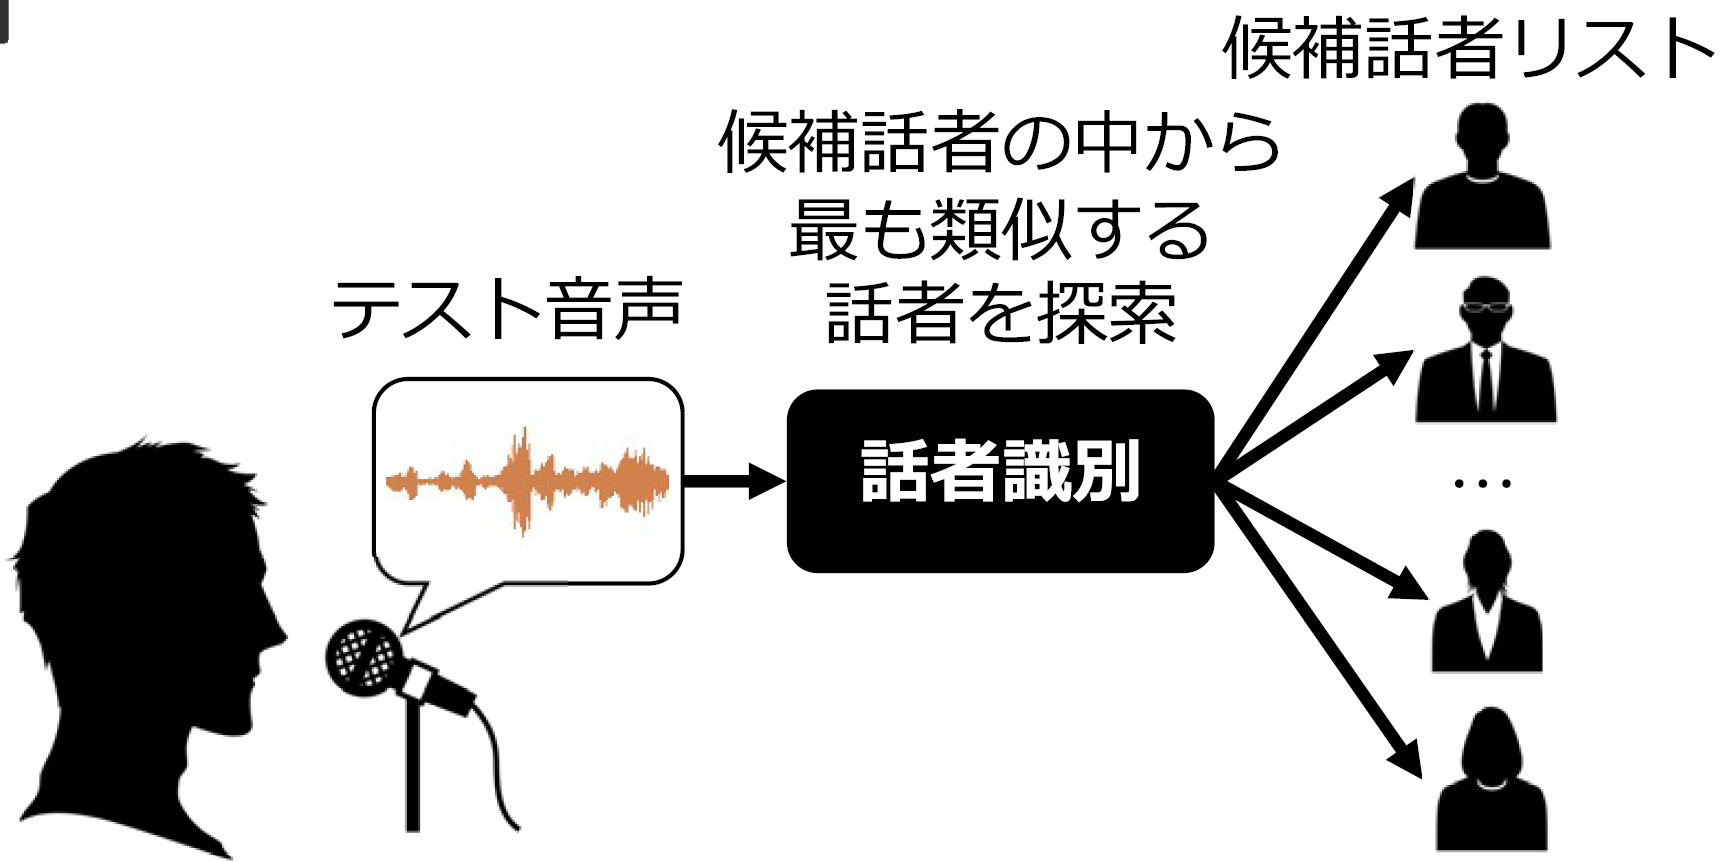
\includegraphics[width=0.8\linewidth]{figures/sd.png}
        \subcaption{話者識別}
    \end{minipage}
    \begin{minipage}{0.9\linewidth}
        \centering
        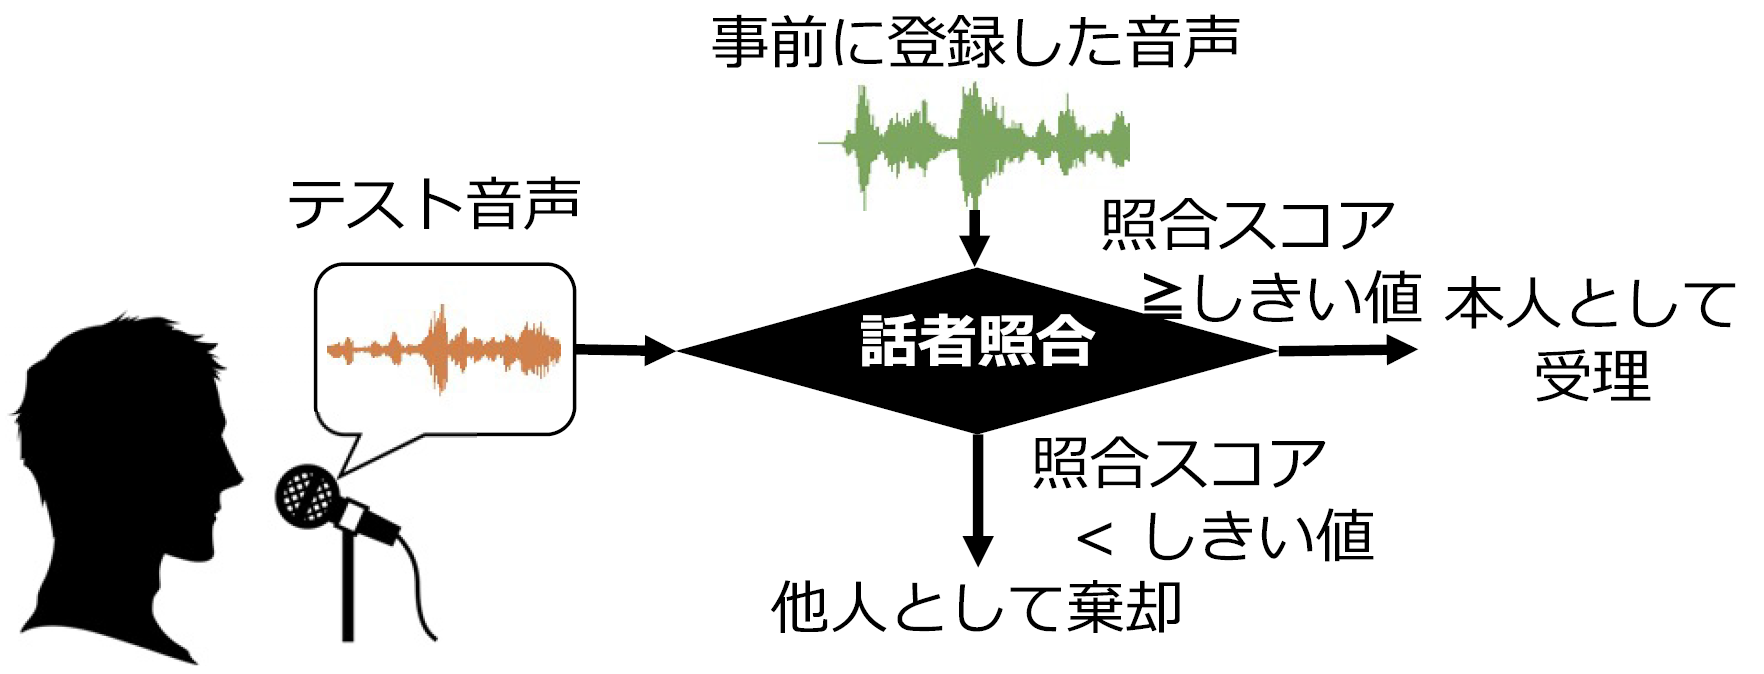
\includegraphics[width=0.8\linewidth]{figures/sv.png}
        \subcaption{話者照合}
    \end{minipage}
    \caption{話者認識の形式 \cite{俵直弘2022}}
    \label{fig:speaker_recog}
\end{figure}

話者識別は事前に登録した複数の候補者の中から提示された音声の話者を探索する1対nの推定問題であるのに対し、
話者照合では,提示された二つの音声が同一話者によるものか否かを推定する1対1の照合問題として定義する \cite{俵直弘2022}。
識別では、未知の話者を既知の話者のデータベースと比較し、最もよく一致する話者を識別結果として与える。
一方で照合では、音声サンプルが主張された人物によって話されたかどうかを判断するタスクと言える \cite{1561284}。
よって、本研究で行うなりすまし偽音声の検出は、話者照合に該当する。

また,話者認識は,登録時と照合時で同じ内容の音声を用いるテキスト依存型(text-dependent)と,
登録時と照合時で異なる内容の音声を用いるテキスト独立型(text-independent)に分類される \cite{俵直弘2022}。
% ASVspoofにおけるなりすまし検出では、テキスト依存型の形式を取っている。
% 読み上げる音声は本人・偽いずれも新聞記事から引用した同一の文章を読み上げているため、
% 実際にSNS上で偽音声による偽情報が投稿された状況から乖離がある。
% よって本研究では、テキスト独立型の話者照合を行う。

\section{既存手法の問題点}
\subsection{コメントと早期検出の相性}
コメントを含めたソーシャルコンテキストを利用する手法に共通した問題点として,ソーシャルコンテキストはユーザの拡散によって生まれる情報であるため早期検出に向かない点が挙げられる.
先述のCVAEによるユーザレスポンス生成器を組み合わせたモデル\cite{ijcai2018-533}では、
ニュース記事を畳み込みニューラルネットワークで特徴化してから隠れ変数を算出し,寄せられたコメントとして尤もらしい単語群を生成することで検出性能が改善されることが報告されている.
しかしながら,TCNN-URGはあくまで尤もらしい単語を生成することに限られ,実際のコメントそのものは生成していない.

また、コメントを考慮するモデルに対して誤った判断へ誘導するコメントを生成する手法も提案されており \cite{9338282}、これは外部から与えられる情報のみに依存する危険性を示している。

\subsection{偽情報媒体の多様化}
近年では、偽情報がもつ媒体が文章に限らず多岐にわたる傾向にある。
記事と画像を併せて発信された情報に対する自動検出手法 \cite{10.1145/3219819.3219903,8919302}はすでに幾つか提案されているものの、
動画や音声など生成技術の発展により対応が必要な媒体の領域が急速に広がっている。

特に既存の偽音声検出手法の多くは、新聞記事を読み上げた人間の音声と合成音声を使ったデータセット \cite{wu15e_interspeech,WANG2020101114}を検出対象としている。
その影響で基本的に音声波形そのものを手法の入力として扱っており、
対象音声がどのような内容の主張を行っているかは考慮に入れていない。

\subsection{検出性能の維持}
偽情報の検出は、偽情報生成側とのいたちごっこが続いている。
元々ニュース記事を検出する場合でも、ドメイン(分野)固有の要因による検出性能の維持の難しさによって、新規ニュースに対して性能維持が難しい点が指摘されている \cite{10.1145/3459637.3482139}ほか、
同一のニューストピックを扱う別々のデータセット間でも、検出性能に大幅な差が出る点もまた指摘されている \cite{10.1007/978-3-030-73696-5_13}。

さらに、GPT-4を始めとするLLMの影響によって偽情報文章の生成が誰でも容易になった点も指摘されている \cite{DWIVEDI2023102642}。
この影響により、今後出現する偽情報はこれまで以上に既存の検出手法を掻い潜りやすくなる点が見込まれる。

